\RequirePackage{fix-cm}
%
\documentclass{svjour3}                     % onecolumn (standard format)
%\documentclass[smallcondensed]{svjour3}     % onecolumn (ditto)
%\documentclass[smallextended]{svjour3}       % onecolumn (second format)
%\documentclass[twocolumn]{svjour3}          % twocolumn
%
\smartqed  % flush right qed marks, e.g. at end of proof
%
\usepackage{graphicx}
%
\usepackage{mathptmx}      % use Times fonts if available on your TeX system
%
%Style
%\documentclass[11pt]{article}
%\usepackage[top=1in, bottom=1in, left=1in, right=1in]{geometry}
%\parindent 22pt

%Packages
\usepackage{adjustbox}
\usepackage{amsmath}
\usepackage{amsfonts}
\usepackage{amssymb}
\usepackage{bm}
\usepackage[table]{xcolor}
\usepackage{tabu}
\usepackage{makecell}
\usepackage{longtable}
\usepackage{multirow}
\usepackage[normalem]{ulem}
\usepackage{epstopdf}
\usepackage{etoolbox}
\usepackage{graphicx}
\usepackage{tabularx}
\usepackage{ragged2e} 
\usepackage{booktabs}
\usepackage{caption}
\usepackage[none]{hyphenat}
\usepackage{fixltx2e}
\usepackage{threeparttablex}
\usepackage[capposition=top]{floatrow}
\usepackage{subcaption}
\usepackage{pdfpages}
\usepackage{pdflscape}
\usepackage{natbib}
\definecolor{maroon}{HTML}{990012}
\usepackage[colorlinks=true,linkcolor=maroon,citecolor=maroon]{hyperref}
\usepackage{endnotes}

\let\footnote=\endnote

\usepackage{tikz}
\usetikzlibrary{shapes}
\usepackage{setspace}
\usepackage{enumerate}
\usepackage{rotating}

%Watermark
\usepackage[printwatermark]{xwatermark}
\usepackage{lipsum}
\definecolor{lightgray}{RGB}{220,220,220}
%\newwatermark[allpages,color=lightgray,angle=45,scale=3,xpos=0,ypos=0]{Preliminary Draft}

%Functions
\DeclareMathOperator{\cov}{Cov}
\DeclareMathOperator{\var}{Var}
\DeclareMathOperator{\plim}{plim}

%Math Environments
%\newtheorem{theorem}{Theorem}[section]
%\newtheorem{claim}[theorem]{Claim}
\newtheorem{assumption}[theorem]{Assumption}
%\newtheorem{definition}[theorem]{Definition}
\newtheorem{hypothesis}[theorem]{Hypothesis}
%\newtheorem{property}[theorem]{Property}
%\newtheorem{example}[theorem]{Example}
\newtheorem{condition}[theorem]{Condition}
%\newenvironment{proof}{\paragraph{Proof:}}{\hfill$\square$}

%Commands
\newcommand\independent{\protect\mathpalette{\protect\independenT}{\perp}}
\def\independenT#1#2{\mathrel{\rlap{$#1#2$}\mkern2mu{#1#2}}}
\newcommand{\overbar}[1]{\mkern 1.5mu\overline{\mkern-1.5mu#1\mkern-1.5mu}\mkern 1.5mu}
\newcommand{\equald}{\ensuremath{\overset{d}{=}}}
\captionsetup[table]{skip=10pt}
%
\begin{document}

\title{The Price of Fringe Benefits when Formal and Informal Labor Markets Coexist}

\author{David Argente$^\dagger$         \and
        Jorge Luis Garc\'{i}a$^*$
}

\institute{$^\dagger$David Argente \at
              5757 South University Avenue. Chicago, IL 60637 \\
              Tel.: +1 773 677 7938\\
              \email{dargente@uchicago.edu}           
           \and
           $^*$Jorge Luis Garc\'{i}a \at
              5757 South University Avenue. Chicago, IL 60637 \\
              Tel.: +1 202 631 8202\\
              \email{jorgelgarcia@uchicago.edu}
}

\date{Received: 7-27-2014 / Accepted: 10-27-2014}
% The correct dates will be entered by the editor


\maketitle

\begin{abstract}
We use the Mexican labor market structure to price the set of fringe benefits that household heads receive when formally employed. We exploit longitudinal, nationally- representative information on household heads who are formal, informal, or switch status at least once in our data. Using monthly labor income and an efficient markets hypothesis, we identify a standard linear model which accounts for time-variant household heads' characte- ristics and household level and time fixed effects. Under the usual strict-exogeneity assump- tion, we find that the price of fringe benefits is approximately 7.9\% of the average monthly labor income of informal workers, or $ \$217$ USD. \\ \\
\textbf{JEL Classification:} D4 \and J3 \and J4 
\keywords{dual labor market \and fringe benefits \and informal labor market}
\end{abstract}

\section{Introduction} \label{section:introduction}
\noindent Most developing countries are characterized by the presence of a large informal sector or large informal labor market (see Figure \ref{figure:figure0}). Workers in this sector usually do not pay taxes, have access to fringe benefits (i.e. social security and health care coverage), or fall under any labor market regulation. The existence of this sector and its recent expansion in many emerging economies has important implications for the functioning of labor markets and for economic growth. In particular, a deeper understanding of what workers consider when deciding which sector to join could greatly improve the efficacy of policies aimed to increase formality.\\
\begin{center}
\begin{figure}[H] 
\caption{Share of Informal Workers by Country}
\label{figure:figure0}
\centering
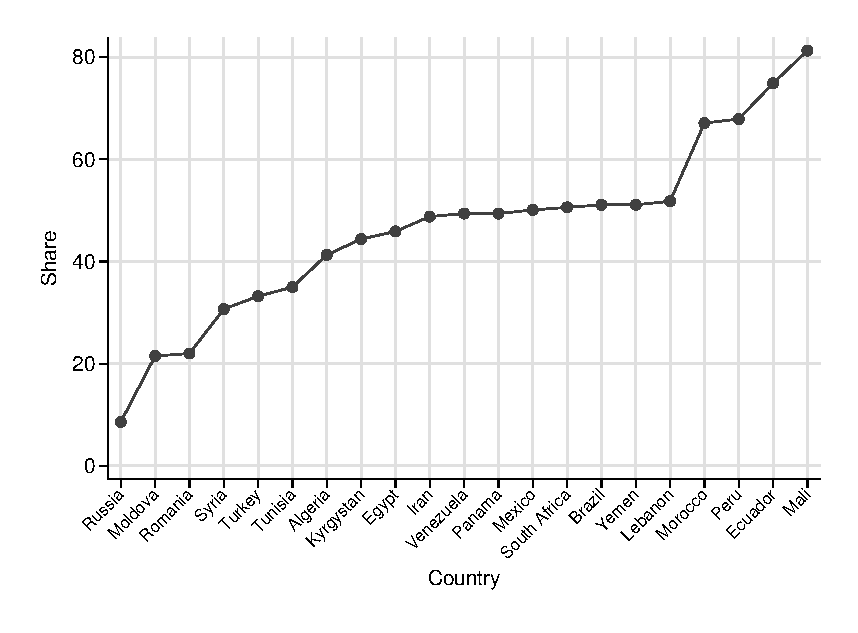
\includegraphics[width=3.5in, height=2in]{cross.eps}
\floatfoot{
\tiny
Note: this figure presents the share of individuals working in the informal labor market by country for the year 2009 (source: \citet{oecd2009}).
}
\end{figure}
\end{center}

\indent How do informal workers price forgone fringe benefits? In this paper, we argue that, in Mexico, informal workers are compensated for the value of lost benefits with higher labor income. We identify the price of these benefits through an approach that combines: i) the Mexican labor market structure, which had $58.3\%$ informal workers in the period 2005-2013; ii) information on monthly labor income; iii) information on individuals who switched from formality to informality or the other way around; iv) an efficient market hypothesis. \\
\indent In particular, if markets are efficient, individuals with identical characteristics should earn the same compensation (inclusive of fringe benefits) regardless of the labor market to which they belong. In other words, if there is perfect mobility between the formal and the informal labor markets, informal workers need to be compensated because there is no law that guarantees them fringe benefits.\footnote{Certain types of workers, such as undocumented immigrants, are more likely to face obstacles to move across markets. In the Mexican context, however, undocumented immigra- tion plays a much smaller role than it does in developed economies. Although there are no official statistics documenting the extent of the presence of undocumented immigrants in the country, the National Institute for Migration estimates that around 400,000 entered the country in 2004 mainly from Central America, a large proportion of them transitioning to the United States (\citet{vazquez2007movimientos}).} The compensation represents how much extra labor income the informal workers get in return for not having fringe benefits. In this paper, we take advantage of the panel structure of the Mexican labor data and exploit the fact that 15\% of the individuals switched from formality to informality between 2005 and 2013. After controlling for time-invariant characteristics, we rely on a efficient market hypothesis and a strict exogeneity assumption to interpret the negative effect of formality on labor income as the price of fringe benefits.\\
\indent In countries such as Mexico, in which the informal sector is a large fraction of the labor force and workers continuously move from formality to informality and the other way around, finding exogenous variation that will induce workers to reallocate from one labor market to the other has proven to be a difficult task. However, one recent example is the introduction of \emph{Seguro Popular}, a program launched to provide health services to uninsured individuals. The program, at first, was thought to be reducing the cost of informality and its critics claimed that a large fraction of the population would switch from formal to informal jobs. Surprisingly, studies have found evidence that the program did not significantly increase informality \citep[see][]{azuara2013informality}. In addition, despite the fact that formal workers have health coverage, a large fraction of them have joined \emph{Seguro Popular}. Figure \ref{figure:seguro} shows that, since its introduction, both formal and informal enrollment rates to the program, although at different levels, have followed similar trends.\\

\begin{figure}[H]
\caption{Share of Beneficiaries \emph{Seguro Popular}, 2005-2013} 
\label{figure:seguro}
\centering
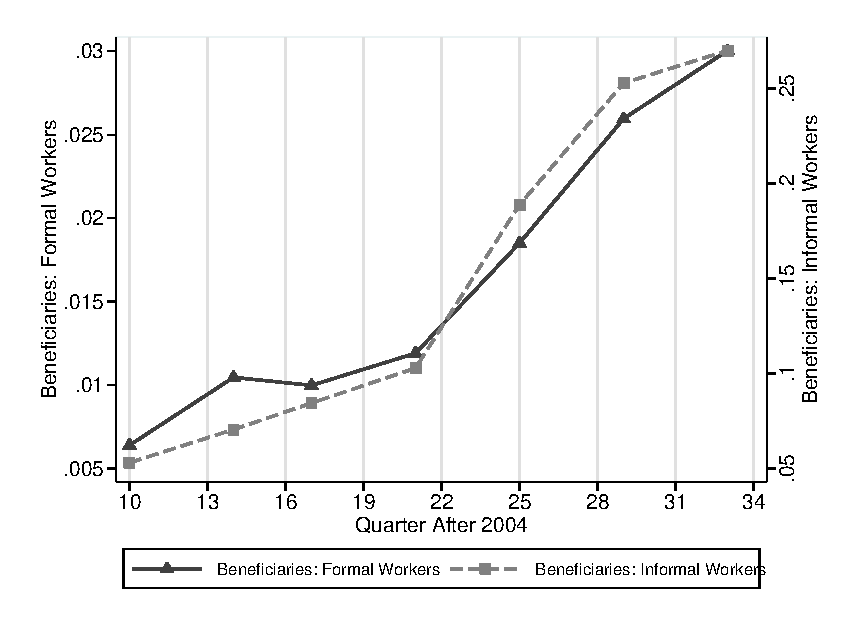
\includegraphics[width=3.5in, height=2in]{policy.eps}
\floatfoot{\begin{tiny}
Note: the graph shows the percent of beneficiaries to \emph{Seguro Popular} that belong to the formal and informal labor markets. \emph{Seguro Popular} is the most prominent component of the Mexican System of Social Protection in Health launched in 2003 to provide health services to uninsured people. The data comes from the National Survey of Occupation and Employment (NSOE).
\end{tiny}}
\end{figure}

\indent Various papers analyze features of markets in which formal and informal labor coexist, but there are few papers pricing fringe benefits.\footnote{\citet{ulyssea2011formal} study whether the formal and informal labor markets are segmented, i.e. if they price the observed and unobserved characteristics of workers in a different way; \citet{ulyssea2010regulation} studies how regulation affects the wage structure, the composition, and the size of the formal and informal labor markets. \citet{carneiro2001modelling} estimate the wage functions for the formal and the informal sectors.}  Juarez: Are Informal Workers Compensated for the Lack of Fringe Benefits? Free Health Care as an Instrument for Formality (unpublished)  and \citet{olson2002workers} ask related questions, but focus on the female labor force. The former estimates the compensation that poor informal female workers receive for the lack of fringe benefits. The latter finds that married female workers accept lower wages in exchange for health benefits.\\
\indent Our data comes from the National Survey of Occupation and Employment (NSOE) collected by the Mexican government. The survey is nationally representative and collects quarterly information on several features of employment conditions for household heads and their respective spouses, as well as socio-demographic characteristics for the period 2005-2013; it has a rotating panel structure in which households are dropped after $5$ observa- tions.\\
\indent Our estimates are calculated using the after-tax labor income based on the assumption that workers consider after-tax labor income when choosing between the informal and formal jobs. Our results indicate that the price of fringe benefits is large and statistically different from zero. We consider these estimates to be relevant, not only to inform policies aiming to increase labor productivity, but also those aimed to improve the employment quality of informal workers. \\
\indent The rest of the paper proceeds as follows. Section \ref{section:data} describes our data. Section \ref{section:markets} describes the formal and informal labor markets in Mexico and defines fringe benefits. Section \ref{section:strategy} presents our empirical findings, and Section \ref{section:results} provides the interpretation and implications of our results. Section \ref{section:finalcomments} concludes.

\section{Data} \label{section:data}
The data we use comes from the National Survey of Occupation and Employment (NSOE) for the period 2005-2013. The survey is nationally representative and collects quarterly information on several features of the employment conditions of heads of households and their respective spouses as well as socio-demographic characteristics. It has a rotating panel structure in which households are dropped after $5$ observations. The questions are identical in each wave of the survey.  For the year 2013, only information for the first quarter is available. Thus, we have an observation span of $33$ quarters after 2004.\footnote{On average, we observe each household head $4.3$ times ($1.2$ s.d.). Information which we can provide under request shows the following: (i) the distribution of observations over time is balanced; (ii) age is the only observable variable that has a significant and economically relevant correlation with the number of periods that the household head is observed.} In our sample, $84\%$ of the household heads are employed, $2\%$ unemployed, and $14\%$ are out of the labor force. In this paper, we focus on the first sub-sample, the employed. In what follows, we explain the map from the raw data to the variables used in our empirical analysis.

\subsection{Information on Income} \label{section:wage}
\begin{figure}[H]
\caption{Median After Tax Labor Income, Formal and Informal Workers, 2005-2013} \label{figure:wage}
  \centering
  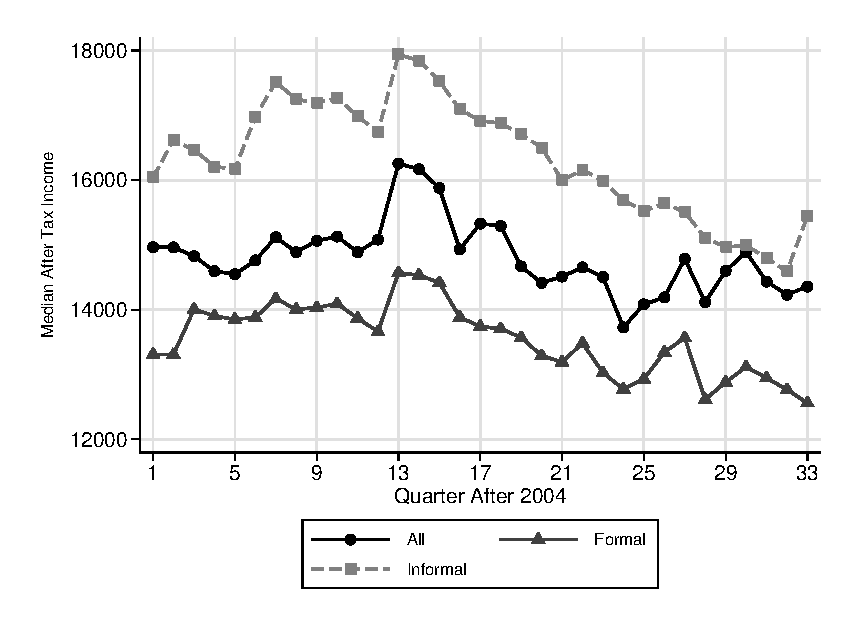
\includegraphics[width=3.5in, height=2in]{income.eps}
\floatfoot{\begin{tiny}
Note: this graph shows the median after-tax labor income of both formal and informal workers for the period 2005-2013. The data comes from the National Survey of Occupation and Employment (NSOE). All income measures were deflated to 2010 pesos using the Consumer Price Index of the Mexican government. The gray bar highlights periods of economic downturn according to Bank of Mexico.  
\end{tiny}}
\end{figure}

\indent We use one question to construct the before-tax monthly labor income variable: ``(in your current job) how much do you currently earn?'' In answering the question, household heads can pick a time scheme between the options (i) monthly, (ii) every 15 days, (iii) weekly, (iv) daily. If the individual answers that he earns on a time scheme other than the monthly scheme, we multiply his reported income as follows: (i) every 15 days, times 2; (ii) weekly, times 4.5; (iii) daily, times 30. By definition, only the formally employed household heads pay taxes or receive credits (individuals with income below a certain threshold which--determined yearly--receive credits). Thus, we calculate an after tax monthly labor income for each household head using the Mexican Government's tax schedule. Figure \ref{figure:wage} displays the time trend of this variable by employment sector. \\
\indent For each household head, we observe the following directly from the survey: age, spouse's age, sex, schooling years, spouse's schooling years, and marital status. In addition, we observe the labor force characteristics of the spouses (i.e. participation and employment). All of the variables are categorical except for schooling years, which is discrete and takes values between 0 (no education) and $24$ (final year of graduate school completed), and age. Table \ref{table:summary2} presents summary statistics for each variable. Importantly, and consistent with the efficient market hypothesis, the mean labor income of formal workers is lower than that of informal workers.\\

\begin{table}[H] 
\begin{threeparttable}
\caption{Basic Descriptive Statistics}
\label{table:summary2}
\centering 
\tiny
\begin{tabular}{lcccc} \hline \hline
 & \multicolumn{2}{c}{Informal} & \multicolumn{2}{c}{Formal} \\ 
 & Mean  & SD  & Mean  & SD  \\  \hline 
Age &    44.465 &     8.407 &    43.025 &     7.966 \\  
Partners' Age &    40.928 &     9.110 &    40.077 &     8.481 \\  
Male &     0.819 &     0.385 &     0.822 &     0.382 \\  
Male Partner &     0.030 &     0.172 &     0.028 &     0.164 \\  
Schooling Years &     7.986 &     4.659 &    11.274 &     4.448 \\  
Partner's Schooling Years &     4.010 &     5.373 &     5.368 &     6.378 \\  
Free Union &     0.158 &     0.364 &     0.097 &     0.296 \\  
Separated &     0.063 &     0.242 &     0.048 &     0.213 \\  
Divorced &     0.027 &     0.163 &     0.040 &     0.195 \\  
Widowed &     0.041 &     0.199 &     0.024 &     0.153 \\  
Married &     0.639 &     0.480 &     0.705 &     0.456 \\  
Single &     0.072 &     0.258 &     0.087 &     0.282 \\  
Employed Partner &     0.979 &     0.145 &     0.973 &     0.163 \\   
Monthly Income & 34,097.524 & 74,850.231 & 17,150.061 & 31,039.965 \\  
\hline \hline \end{tabular}\begin{tablenotes}[flushleft]
\tiny
\item Note: this table contains summary statistics for household heads observed in the National Survey of Occupation and Employment (NSOE). The statistics describe the observable characteristics of the household heads the first time they were observed in the sample. Individuals are classified as formally employed if they have health insurance from the Mexican Institute of Social Security or the Institute of Security and Social Services for the State Workers. In order to receive either service, the worker must pay labor income taxes through his employer. Otherwise he or she is classified as informal employee.\\
\end{tablenotes}
\end{threeparttable}
\end{table}

\indent In our empirical analysis, we consider all household heads aged $30$ to $60$ years old (prime working age). We identify the household head based on a survey question which asks the relationship to the household head for each individual. This status is verified in each of the $5$ waves. We focus on household heads because they are usually employed and we do not model the decision to participate in the labor market. Our final sample includes $419,188$ individual household head observations and $1,278,591$ pooled observations.\footnote{$82\%$ of the household heads we observe are male.}\\

\section{The Formal and Informal Labor Markets} \label{section:markets}
\indent Formal employment, which happens in the formal labor market, is a working relationship between a employer and employee that is fully under governmental regulation and taxation. Informal employment is any employment that does not fall under governmental regulation and taxation.\\
\indent Mexican federal labor law mandates formal employers to provide a set of fringe benefits which are often considered to cover basic individual and family needs. This includes maternity leave, overtime pay, disability income protection, retirement benefits, sick leave, vacations (paid and non-paid), social security, and profit sharing, and a number of other benefits.\footnote{Appendix \ref{section:fringe} includes a full list of the benefits mandated by Mexican law. Formal workers are recipients of these benefits.} For this reason, we classify a household head as formally employed if he or she works and receives health insurance and social security services through the Mexican Institute of Social Security or the Institute of Services and Social Security for the State Workers. The former provides services to private industry employees and the latter to government employees. In order to receive either service, individuals must be registered as contributors and pay labor income taxes. Firms that do not register employees are subject to a variety of fines. This registration is the unique channel through which the government learns that an employee is working.\footnote{Unfortunately, the official registry is not public. We use self-reported status instead.} The firm declares the labor income of the employee, and the government taxes the firm accordingly. Then, the firm subtracts this tax from the employee's labor income. Notably, self-employed individuals can register themselves as firms, pay taxes, and receive benefits as if employed by a firm. \\
\indent We use the following question to define formal employment or \emph{formality}: ``do you have access to medical aid in...?'' If the household head answers either Mexican Institute of Social Security or Institute of Services and Social Security for the State Workers, we consider him or her to be formally employed. Figure \ref{figure:figure3} describes the participation of employed household heads in the formal labor market over time and over the life cycle. Participation over time is stable for two reasons: (i) no structural changes have increased or decreased the participation rates in either the formal or the informal labor markets; (ii) the employment rate in Mexico for the period 2005-2013 is very stable: $97\%$ of household heads are employed with a standard deviation of $16\%$.\footnote{At least two explanations can account for the shape of the participation rate in the formal labor market over the life cycle. First, formal jobs could require higher human capital, and older individuals suffer from human capital depreciation. Second, relatively old individuals may take jobs in the informal sector because of more flexible schedules that enable them to allocate time to other activities such as leisure. Both stories trace back to old discussions in the Economics literature. See \citet{carlinger1982wagesolderman} for a discussion of labor market characteristics as the age of the individuals differ and \citet{heckman1976life} for a study of a life-cycle model of learning, earnings, and consumption.}

\begin{figure}[H]
\centering
\caption{Formal Employment in Mexico, 2005-2013}
\label{figure:figure3}
\begin{subfigure}{.4\textwidth}
  \centering
  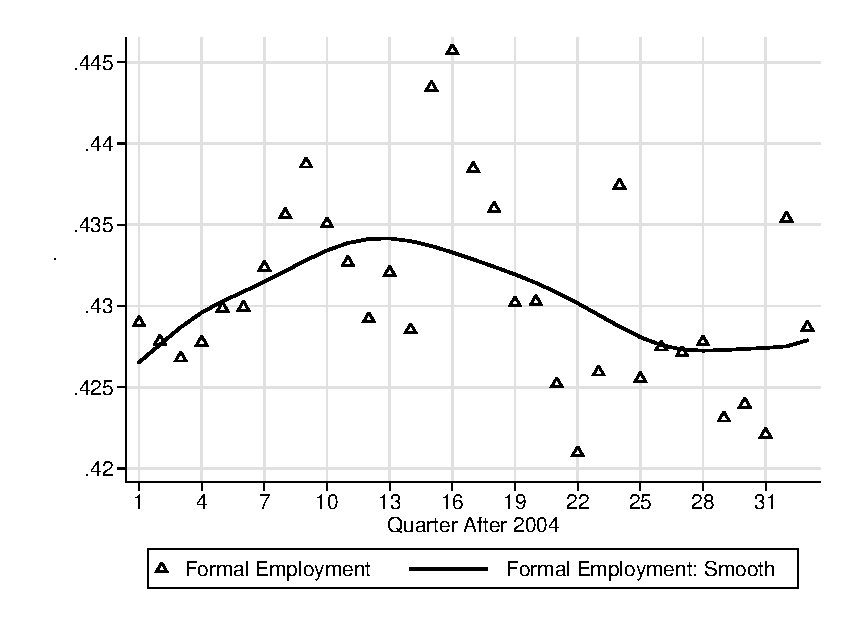
\includegraphics[width=1.5in, height=1in]{formaltime.eps}
  \caption{Over Time}
\end{subfigure}%
\begin{subfigure}{.4\textwidth}
  \centering
  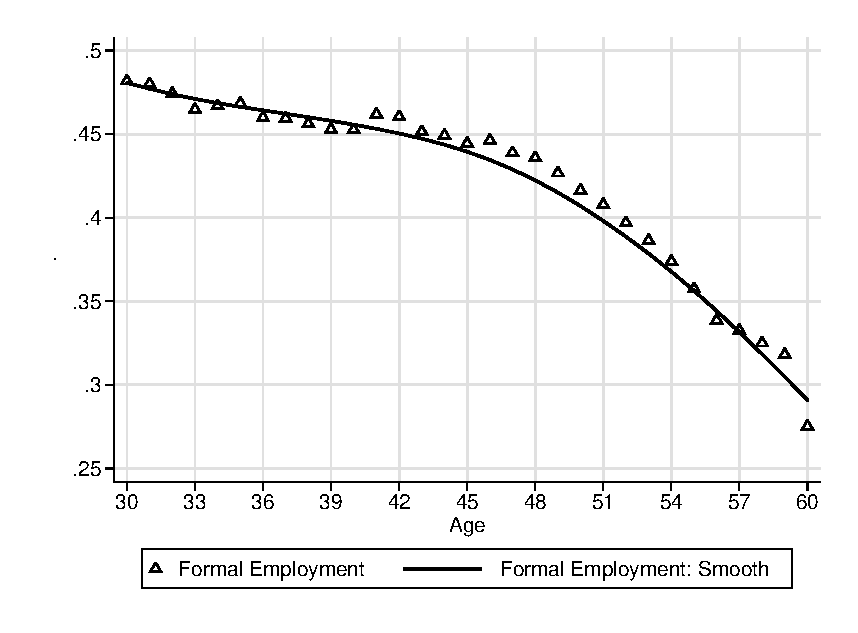
\includegraphics[width=1.5in, height=1in]{formallcycle.eps}
  \caption{Over the Life Cycle}
\end{subfigure}
\floatfoot{\begin{tiny}
Note: a worker is formal if he has health insurance and social security services from the Mexican Institute of Social Security or the Institute of Security and Social Services for the State Workers. In order to receive either service, the worker must pay labor income taxes through their employer. We deflate all income measures to 2010 pesos using the Consumer Price Index of the Mexican government. The data comes from the National Survey of Occupation and Employment (NSOE).
\end{tiny}}
\end{figure}

\section{Empirical Strategy} \label{section:strategy}
Since our estimation relies on an efficient market hypothesis, our first step is to check the extent to which it holds in our sample. If the efficient market hypothesis holds, then workers should be indifferent between working in the formal and informal sectors. If this is the case, we should observe that moving from the formal to the informal sector happens as often as a move in the opposite direction. To check this, we divide the ``switchers'', individuals who switch (in our window of observation) from one labor market to the other without spending time as unemployed, into three different groups: i) individuals who started in the formal sector and switched to the informal sector; ii) individuals who started in the informal sector and switched to the formal sector; iii) individuals who switched across sectors several times.\footnote{Recall that in our sample, we observe the same worker an average of 4.3 times and a maximum of 5.} Table \ref{table:switch} shows that 15.4\% of the heads of household in our data switch labor markets at some point. Of the switchers, 42.2\% started as formal and switched to informal and 42.9\% started as informal and switched to formal.\footnote{The rest of the individuals switch more than one time across the two sectors. We divide them in three categories to ease interpretation. Since we observe individuals at most 5 times, there are $2^5$ patterns which they could follow and it is hard to analyze this in an intuitive way. Instead, these three categories show that, in fact, two patterns encompass all the switches. Importantly, two of the categories show evidence on similar frequencies across switches between formality and informality and the other way around.}  

\begin{table}[H] 
\begin{threeparttable}
\caption{Fraction of Head of Households Switching Sectors, 2005-2013}
\label{table:switch}
\centering 
\tiny
\begin{tabular}{lcc} \hline \hline
 & Mean  & SD  \\  \hline 
Switches &     0.154 &     0.361 \\  \hline
To Informal &     0.424 &     0.494 \\  
To Formal   &     0.429 &     0.495 \\  
\hline \hline \end{tabular}
\begin{tablenotes}[flushleft]
\tiny
\item Note: this table shows the fraction of workers that switch from one labor market to the other between 2005-2013. The data comes from the National Survey of Occupation and Employment (NSOE).
\end{tablenotes}
\end{threeparttable}
\end{table}

\indent Having shown that in our data, switching from informality to formality happens as often as switching from formality to informality, we now turn to show that the labor income of the three groups does not significantly differ. Put differently, we want to test, in order to make our efficient market hypothesis more credible, that specific types of switches are not associated with labor income gains. To do this, we regress a set of indicators for each type of switcher on our measures of monthly labor income. Table \ref{table:smodels} displays the results of these calculations under different specifications. Column 3 shows that the difference between the labor income of the three types is close to zero. We then compute the returns to formality of the switchers with (column 4) and without (column 2) controls for the switcher type. Importantly, the returns to formality do not significantly differ between these two specifications, and the coefficient is negative and significantly different from zero --which aligns with our main empirical findings discussed next in this section.

\begin{table}[H] 
\begin{threeparttable}
\caption{Linear Models with Switching Indicators}
\label{table:smodels}
\centering 
\tiny
\begin{tabular}{lcccc} \hline \hline
 & (1) & (2) & (3) & (4) \\ \hline
Formal &  & -0.04548*** &  & -0.04415*** \\
 &  & (0.00382) &  & (0.00387) \\
Switch to Formal &  &  & 0.01523** & 0.01229** \\
 &  &  & (0.00595) & (0.00596) \\
Switch to Informal &  &  & 0.00062 & 0.00418 \\
 &  &  & (0.00588) & (0.00589) \\
2-5 Co-workers & 0.05669*** & 0.06683*** & 0.05704*** & 0.06670*** \\
 & (0.00819) & (0.00826) & (0.00819) & (0.00826) \\
6-10 Co-workers & -0.05050*** & -0.02923*** & -0.04934*** & -0.02924*** \\
 & (0.00865) & (0.00888) & (0.00865) & (0.00887) \\
11-15 Coworkers & -0.10785*** & -0.08250*** & -0.10643*** & -0.08247*** \\
 & (0.00969) & (0.00998) & (0.00970) & (0.00998) \\
16-50 Co-workers & -0.15065*** & -0.12127*** & -0.14886*** & -0.12114*** \\
 & (0.00813) & (0.00856) & (0.00814) & (0.00856) \\
$>$50 Co-workers & -0.23406*** & -0.20118*** & -0.23181*** & -0.20092*** \\
 & (0.00785) & (0.00836) & (0.00787) & (0.00836) \\
Age & 0.24550* & 0.24945* & 0.23231 & 0.23502 \\
 & (0.14679) & (0.14674) & (0.14727) & (0.14722) \\
Partner's Age & -0.00326*** & -0.00323*** & -0.00327*** & -0.00324*** \\
 & (0.00036) & (0.00036) & (0.00036) & (0.00036) \\
Male & 0.35589*** & 0.35426*** & 0.35521*** & 0.35365*** \\
 & (0.01277) & (0.01277) & (0.01277) & (0.01277) \\
Schooling Years & -0.00125*** & -0.00135*** & -0.00123*** & -0.00133*** \\
 & (0.00038) & (0.00038) & (0.00038) & (0.00038) \\
Free Union & 0.02210 & 0.02158 & 0.02146 & 0.02116 \\
 & (0.03150) & (0.03150) & (0.03149) & (0.03150) \\
Separated & 0.01780 & 0.01865 & 0.01775 & 0.01873 \\
 & (0.04521) & (0.04517) & (0.04521) & (0.04517) \\
Divorced & 0.09595 & 0.09606 & 0.09626 & 0.09601 \\
 & (0.06223) & (0.06199) & (0.06227) & (0.06202) \\
Widowed & 0.08004 & 0.07885 & 0.08049 & 0.07913 \\
 & (0.10689) & (0.10674) & (0.10685) & (0.10670) \\
Married & -0.01402 & -0.01355 & -0.01444 & -0.01397 \\
 & (0.03129) & (0.03128) & (0.03128) & (0.03128) \\
Constant & 6.82986*** & 6.78857*** & 6.97563*** & 6.94826*** \\
 & (1.55758) & (1.55705) & (1.56306) & (1.56256) \\ \hline
 Time Fixed Effects & Yes &  Yes &  Yes &  Yes \\
Observations & 224,584 & 224,584 & 224,584 & 224,584 \\ \hline \hline
\end{tabular}
\begin{tablenotes}[flushleft]
\tiny
\item Note 1: robust standard errors in parentheses: *** p$<$0.01, ** p$<$0.05, * p$<$0.10.
\item Note 2: this table displays the results of regressions of a set of indicators for each type of switcher on our measures of monthly labor income. Column 3 shows that the difference between the labor income of the three types is close to zero. We then compute the returns to formality of the switchers with (column 4) and without (column 2) controls for the switcher type. The data comes from the National Survey of Occupation and Employment (NSOE).
\end{tablenotes}
\end{threeparttable}
\end{table}

\indent Since our previous exercise only considers individuals who switch sectors at some point, we now estimate the returns to formality using the entire sample. Our estimates, under the efficient market hypothesis and strict exogeneity,\footnote{Strict exogeneity is the generalization of exogeneity for the case of linear models with longitudinal data. Mathematically, we express it as follows: $\mathbb{E} \left[ \varepsilon_{it} | F_{i,t} \right] = 0$ for all individuals $i$ and all time periods $t$.} can be interpreted as the price of fringe benefits. We use the following linear model: 
\begin{equation}
Y_{i,t} = \kappa + \beta F _{i,t} + \lambda_{i} + \phi_{t} + \epsilon_{i,t} \label{eq:first}
\end{equation}
where $Y_{i,t}$ and $F_{i,t}$ are the monthly labor income and the formal employment status of household head $i$ at time $t$, respectively. $\kappa$ is a constant, $\lambda_{i}$ denotes individual fixed effects, and $\phi_{t}$ time fixed effects. Since we control for all time-invariant characteristics, individual transitions across markets enable us to identify the effect of formality. This sheds light on the impact of formality on individual outcomes since most characteristics remain fixed within our observation window while only formality status changes. In addition, we control for other observable time-varying characteristics such as age, schooling years, marital status, and the size of the firm in which the household head works.\\

\section{Results} \label{section:results}
Our results are presented in Table \ref{table:femodels} where we display various specifications adding demo- graphic controls and individual and time fixed effects. Our preferred estimates, in column 5, include individual and time fixed effects and controls for the firm size.\footnote{Column 3 and column 4 show the results with and without time fixed effects. The results do not significantly change since a large portion of the variation is explained by the individual fixed effects.} The coefficient of our formality indicator shows that the average effect of formality on monthly labor income of household heads is -8\%, \emph{ceteris paribus}, meaning all other household head characteristics are fixed.\footnote{\citet{heckman2013causal} explain the notion of \emph{ceteris paribus} and define what \emph{fixing} means in Economics and how it differs from \emph{conditioning} in Statistics.} If markets are efficient, individuals with identical characteristics should have the same compensation (inclusive of fringe benefits) in the formal and informal labor markets. Thus, under that assumption, this procedure enables us to interpret our estimates as the average monthly price of fringe benefits.\\
\indent Consider the following example. Take a formally employed individual. He reports a total labor income of $\$2,000$ for December, 2012. However, his employer provides him with a set of fringe benefits that an informal employee does not receive. If these two household heads only differ by formal versus informal employment and markets are efficient, an informally employed individual requires a  cash compensation in order to work in the informal market. According to our estimation, an informal worker would require $\$2,000 + \$2,000*.079$ to work in December 2012. Since on average an informal employee earns $34,097.52$ MXN (2010), a simple calculation suggests the average monthly price of fringe benefits is $2,693.$ MXN (2010).\\  
\begin{table}[H] 
\begin{threeparttable}
\caption{Linear and Linear Fixed Effects Models}
\label{table:femodels}
\centering 
\tiny
\begin{tabular}{lccccc} \hline \hline
 & (1) & (2) & (3) & (4) & (5) \\ \hline
Formal &  & -0.28994*** & -0.09718*** & -0.09673*** & -0.07910*** \\
 &  & (0.00164) & (0.00366) & (0.00366) & (0.00383) \\
2-5 Coworkers &  &  &  &  & 0.07625*** \\
 &  &  &  &  & (0.00446) \\
6-10 Coworkers &  &  &  &  & 0.05417*** \\
 &  &  &  &  & (0.00549) \\
11-15 Coworkers &  &  &  &  & 0.03285*** \\
 &  &  &  &  & (0.00607) \\
16-50 Coworkers &  &  &  &  & 0.00393 \\
 &  &  &  &  & (0.00558) \\
$>$50 Coworkers &  &  &  &  & -0.00550 \\
 &  &  &  &  & (0.00582) \\
Age & 0.12675* & 0.11209* & -0.18281 & -0.18171 & -0.20678 \\
 & (0.06850) & (0.06779) & (0.29515) & (0.29501) & (0.30130) \\
Partner's Age & -0.00322*** & -0.00255*** & -0.00548*** & 0.00273 & 0.00208 \\
 & (0.00017) & (0.00017) & (0.00204) & (0.00261) & (0.00259) \\
Male & 0.28171*** & 0.28652*** & -0.39365* & -0.41047** & -0.39794** \\
 & (0.00550) & (0.00547) & (0.20355) & (0.18245) & (0.19731) \\
Schooling Years & -0.00803*** & 0.00060*** & -0.06310* & -0.06293* & -0.06616* \\
 & (0.00017) & (0.00018) & (0.03583) & (0.03439) & (0.03481) \\
Free Union & 0.08092*** & 0.05709*** & 0.04139 &  & 0.02703 \\
 & (0.01523) & (0.01512) & (0.19179) &  & (0.20179) \\
Married & 0.01397 & 0.01775 & -0.06259 & -0.08864 & -0.05447 \\
 & (0.01512) & (0.01502) & (0.11456) & (0.15395) & (0.12491) \\
Seperated & 0.09260*** & 0.08177*** &  & -0.02309 &  \\
 & (0.02265) & (0.02241) &  & (0.19548) &  \\
Divorced & 0.02274 & 0.04410 &  &  &  \\
 & (0.02934) & (0.02911) &  &  &  \\
Widowed & 0.08890** & 0.08103* &  &  &  \\
 & (0.04242) & (0.04220) &  &  &  \\
Constant & 8.05017*** & 8.29659*** & 12.78781*** & 12.24017*** & 12.46080*** \\
 & (0.72694) & (0.71933) & (3.12531) & (3.12017) & (3.18795) \\ \hline
 Individual Fixed Effects & No  & No & Yes & Yes & Yes \\
 Time Fixed Effects & No  & No & No & Yes & Yes \\
 Observations & 1,278,591 & 1,278,591 & 419,188 & 419,188 & 415,560 \\ \hline \hline
\end{tabular}
\begin{tablenotes}[flushleft]
\tiny
\item Note 1: robust standard errors in parentheses (clustered at individual level): *** p$<$0.01, ** p$<$0.05, * p$<$0.10.
\item Note 2: this table shows the results of various specifications adding demographic controls and fixed effects. Our preferred estimates, in column 5, include individual and time fixed effects and controls for the firm size. Column 3 and column 4 show the results with and without time fixed effects. The data comes from the National Survey of Occupation and Employment (NSOE).
\end{tablenotes}
\end{threeparttable}
\end{table}

\subsection{Discussion} \label{section:discussion}
\indent In Mexico, firms that do not register employees as contributors are subject to a variety of fines. If firms hiring informal workers take into account the expected cost of hiring an informal worker, then the difference between the informal and formal labor income also includes the expected fine employers anticipate to pay. In this case, our estimates could be considered as a lower bound of actual fringe benefits. On the other hand, our results are only indicative of the price of the fringe benefits mandated by Mexican law. Due to data limitations, our strategy to price of fringe benefits does not control for immediate and delayed benefits, ``longer working hours'', or job characteristics. Thus, the price we estimate bundles the series of benefits described in Appendix \ref{section:fringe} plus any other compensation a worker requires to join either labor market sector. 

\section{Conclusion} \label{section:finalcomments}
\noindent Considering that $58.3\%$ of Mexican workers are employed informally, understanding how and why these workers choose informality is of crucial importance for policymakers who design policies to reduce the size of this sector. To this end, in this study, we provide estimates of the price of fringe benefits that formally employed household heads receive. Our estimates are the result of combining information on monthly labor income for heads of households and the structure of the Mexican labor market with an efficient markets hypothesis. In particular, taking advantage of a large longitudinal dataset, we estimate the effect of formality for heads of households who switch from one sector to the other between 2005 and 2013. We interpret the after-tax labor income differential we found as the price of fringe benefits that informally employed household heads receive. Given the size of our estimates ($7.9\%$), future research should try to disentangle and quantify the different contributions to the compensation gap between formal and informal workers. \\ \\


\noindent \textbf{List of Abbreviations} \\
NSOE \indent National Survey of Occupation and Employment

\begin{acknowledgements}
We are grateful to the editor, Pierre Cahuc, and to two anonymous referees for insightful feedback. We thank  Andrea Ar\'{e}valo, Cristi\'{a}n Dagnino, Munseob Lee, Bruce Meyer, Casey Mulligan, Yona Rubinstein, Joshua Ka Chun Shea, and Yike Wang for helpful comments and Pedro R. Garc\'{i}a for information and thoughts about the labor income taxation laws in Mexico. We also thank Sneha Elango for outstanding research assistance. All remaining errors are our own.
\end{acknowledgements}

\small
\noindent \textbf{Competing Interests} ‘The IZA Journal of Labor
Economics is committed to the IZA Guiding
Principles of Research Integrity. The authors declare
that they have observed these principles.

\begingroup
\parindent 0pt
\parskip 2ex
\def\enotesize{\normalsize}
\pdfbookmark{Endnotes}{Endnotes}
\theendnotes
\endgroup

% BibTeX users please use one of
%\bibliographystyle{spbasic}      % isn't compiling the bibliography
\bibliographystyle{chicago}
\bibliography{lmx}

\renewcommand{\thesection}{\Alph{section}}
\setcounter{figure}{0}  \renewcommand{\thefigure}{A1.\arabic{figure}}
\setcounter{table}{0}   \renewcommand{\thetable}{A1.\arabic{table}}
\setcounter{section}{0}
\section{Appendix} \label{section:appendix}
\subsection{Fringe Benefits} \label{section:fringe}
The complete list of the fringe benefits mandated by the federal labor law in Mexico is the following:
\begin{enumerate}[(a)]
\item Pregnant women do not work during twelve weeks centered around the delivery date and preserve their job and their complete salary package 
\item Labor income is paid in cash
\item Extra hours are paid double\footnote{Day shifts (between $6$ a.m. and $6$ p.m.) are $8$ hours long while night shifts (between $6$ p.m. and $6$ a.m.) are $7$ hours long. Shifts that overlap between day and night shifts are $7.5$ hours long. The hours that go beyond the shift duration are extra hours.} 
\item In the case of job-related accidents or diseases, workers preserve their job and their full salary package during a period that secondary laws determine in each case
\item One day off for every six days of work with the payment of full labor income
\item Six vacation days per year with the payment of full labor income
\item Two additional vacation days for every year employed in the same firm, with the payment of full labor income
\item Two additional vacation days after the fourth year employed in the same firm, with the payment of full labor income
\item Two additional vacation days for every five years employed in the same firm, with the payment of full labor income
\item $25\%$ vacation bonus, i.e. workers receive $125\%$ of their labor income during vacation days
\item Workers receive their full labor income and do not work during observed holidays\footnote{As of 2013, there were seven observed holidays: (i) January the 1st, (ii) the first Monday of February to commemorate the Constitution's day, (iii) the third Monday of March to commemorate the birth of Benito Ju\'{a}rez (Mexican president during the 19th century); (iv) Worker's Day (May 1st); (v) Independence Day (September 16th); (vi) the third Monday of November to commemorate the Mexican Revolution; (vii) Christmas (December 25th).} 
\item $30$ minutes break for each working shift, with the payment of full labor income
\item $25\%$ compensation for working on Sundays, i.e. workers receive $125\%$ of their labor income when they work on Sundays
\item $15$ days of additional labor income at the end of each working year
\item $8\%$ of the total before-tax yearly profits of the firms are divided between all its workers. The amount that each worker receives is an increasing function of his labor income and the number of days that he works in the firm the current year
\item Employers, employees, and the government jointly cooperate to pay for a basket of health services, provided either by the Mexican Institute of Social Security or the Institute of Services and Social Security for the State Workers
\item Employers, employees, and the government jointly contribute to a savings account for retirement and housing. The three parties accumulate resources so that the workers can both have savings for the retirement and funds to buy housing. They can access the former after retirement and the latter after a period of time that enables them to buy a housing property through a governmental system or to complement external savings or mortgages to buy private housing.\footnote{Another common benefit that formal workers have, although the law does not enforce it, is access to a savings fund which works as follows. The firm discounts certain amount from the worker's labor income and invests it in a worker savings fund. For each worker, the firm invests a similar amount from that discounted from the worker's labor income. This amount is called firm's contribution. At the end of the year, the worker receives the total amount discounted over the year together with the firm's contribution and interest payments.}\\
\end{enumerate}

\begingroup
\parindent 0pt
\parskip 2ex
\def\enotesize{\normalsize}
\pdfbookmark{Endnotes}{Endnotes}
\theendnotes
\endgroup

\end{document}
